In the previous chapter the terms "immersion", "presence" (and "hand presence") and even "virtual reality" are used in a loose manner. In academia, however, these terms are problematic because of the wide range of fields in which they are used, with very specific and not always similar meanings. Here we will frame the virtual environment constraints problem in existing theories and ground these terms in the academic literature.

\section{Virtual Reality}
\label{sec:vrDef}

Virtual Reality is frequently thought of in terms of a collection of hardware devices commonly associated with the medium: head mounted displays, tracking devices, etc... One such definition focus on the technology is Coates':

\begin{displayquote}
\textit{"Virtual Reality is electronic simulations of environments experienced via head mounted eye goggles and wired clothing enabling the end user to interact in realistic three-dimensional situations."} As cited in \parencite{Steuer1992}.
\end{displayquote}

However, for the purposes of various fields of knowledge such as communication research and for software developers, \parencite{Steuer1992} argues that the medium needs a definition with an experiential focus instead of a technological one. Steuer works his way from Gibson's definition of presence "the sense of being in an environment" (as cited in \parencite{Steuer1992}) through telepresence as "the experience of presence in an environment by means of a communication medium" \parencite{Steuer1992} and finally arrives at a definition of virtual reality independent of any technological specifics as:

\begin{displayquote}
\textit{A virtual reality is a real or simulated environment in which a perceiver experiences a sense of being in that environment by means of a communication medium.} \parencite{Steuer1992}
\end{displayquote}

\section{Immersion}
\label{sec:immersion}

Slater provides a definition of immersion based on "the actions we know to carry out in order to perceive" or Sensorimotor Contingencies (SC), from behavioural and brain scientist O'Regan and Noë (as cited in \parencite{Slater2009}). Examples of SCs are turning one's moving your eyes to look in a certain direction, reaching out with our hand to feel a surface with our sense of touch or turning our head sideways to align one of our ears with the direction that a sound seems to come from in order to hear it more clearly. Note that SCs relate to all of our senses. Slater's definition of immersion is:

\begin{displayquote}
\textit{Immersion is a property of the actions that the user can take that result in changes in perception (Valid Sensorimotor Actions), or changes to the environment (Valid Effectual Actions) within a system.} \parencite{Slater2009}
\end{displayquote}

This means that immersion is an objective property of virtual reality systems that can be used to compare them. A system can be said to be more immersive than another system if the first system's set of Valid Actions (Valid Sensorimotor Actions + Valid Effectual Actions) is greater than the second system's set.

\todo[inline]{Compare Oculus, Vive and PS VR?}

\section{Place Illusion and Plausibility Illusion \textit{in lieu of} Presence}
\label{sec:PIandPsi}

In the context of Virtual Reality, the term presence is usually used meaning the "sensation of being in the virtual world" \parencite{Schuemie2001}. To avoid possible confusion due to the multiple definitions and theories related to the term "presence" (see \parencite{Schuemie2001} for an overview), we will instead use the terms Place Illusion (PI), "the illusion of being in a place in spite of the sure knowledge that you are not there", and Plausibility Illusion (Psi), "the illusion that what is apparently happening is really happening in spite of the knowledge that it is not", proposed in \parencite{Slater2009}.

These definitions are however rather unspecific on their own and require further explanation to be useful. In an interview, Slater describes PI as "the result of using your body to perceive in the way that you would normally" and Psi as "the result of the observed coherence of the world and the extent to which it matches our expectations about how it works" \parencite{Slater2015}.

Considering only these new descriptions, one might wonder if having a virtual body is in fact connected to PI at all. Without having a virtual body, would it still be possible to perform the same actions with our real body to produce the same changes in our sensory displays? We could turn our real head to look around, but when looking down, we wouldn't see our body. We could reach out with our read hand and feel an object when we touch it, but our hand would not occlude the view of the object we are touching. Our body is a constant in our perception, the actions we perform to perceive the world are always conditioned by the fact that our body is always there. Therefore, we consider that having a virtual body that synchronously follows the movements of our real body is part of PI. In fact, Slater points at the body as being related to both PI and Psi:

\begin{displayquote}
\textit{"The body is a focal point where PI and Psi are fused. As we have argued the action involved in looking at your own body provides very powerful evidence for PI (your body is in the place you perceive yourself to be). However, this virtual body is not yours, it is a representation of you. In principle you have no control over what it does. Now suppose you move your limbs and you see the limbs of this virtual body move in synchrony. This is a very powerful event in the external world that clearly relates to you – a correlation between proprioception and visual exteroception. Further, it is likely that there would be some degree of ownership over this virtual body – it comes to ‘really’ seem to be your body (even though you know it cannot be)."} \parencite{Slater2009}
\end{displayquote}

The connection between the body and Psi that Slater is describing here is subtle. In \parencite{Slater2009} he points out that a key component of Psi is that events in the virtual environment refer directly to you. A straightforward example that Slater himself uses is virtual characters acknowledging you and acting in a believable way towards you. But the virtual body you see in the space you occupy is not your own, it is also part of the virtual world and by reacting to you movements it establishes a relation to you that includes you in that virtual world. Since you are real, your inclusion in the virtual world makes it more real.

Interestingly, Slater doesn't explicitly relate the physics of the virtual world with either PI or Psi. We would argue though, that because of our knowledge of how real physical objects work, our expectation will be that the objects that we see in virtual reality behave the same way, therefore we consider physics to be related to Psi. This includes how our virtual body should interact with the virtual environment. A dissonance between the way the real world works and the way the virtual world works would remind us of the irreality of the experience, which would be a break of Psi. If the world we perceive doesn't work like the real world, it cannot be the real world. 

We should emphasize that both PI and Psi are subjective experiences. In the same virtual reality, a user that only looks around in a virtual environment will have a very different degree of PI than one that moves around a lot and runs into a real wall, tries to touch a virtual object and realizes they can't feel it with their sense of touch. In regards to Psi, the user's expectations of the world will be different based on their knowledge of it. For instance: a chemist will have very different expectations about a virtual chemistry lab than a farmer.

Slater's work is not developed specifically for VR games. His research is concerned with how to elicit realistic behaviors in virtual situations, which is extremely relevant in order to use VR for therapeutic purposes or to explore moral issues. The degree of PI and Psi that games might be interested in producing might be different. Some genres, like horror games, might benefit from having realistic virtual environments that produce a high degree of Psi, while other genres might have no interest in such realism and in those cases the effort will have to be in producing suspension of disbelief in the player and maintaining a coherent world that matches the expectations set by the tone of the game.

\todo[inline]{Mention PI as the spatial experience of being inside a world \parencite{Kilteni2012}?}

\section{Sense of Embodiment}
\label{sec:embodiment}

In dealing with virtual hands, we are considering what connection one might experience towards a virtual body. \parencite{Kilteni2012} propose the notion of Sense of Embodiment (SoE) to address the issue of "whether it is possible to experience the same sensations towards a virtual body as toward a biological body":

\begin{displayquote}
\textit{"SoE toward a body B is the sense that emerges when B's properties are processed as if they were the properties of one's own biological body."}
\end{displayquote}

Kilteni et al. further explain SoE in terms of three subcomponents:

\begin{displayquote}
\begin{itemize}
\item \textit{Sense of Self-Location: "one's spacial experience of being inside a body."}
\item \textit{Sense of Agency: "the sense of having global motor control, including the subjective experience of action, control, intention, motor selection and the consious experience of will"} (Blanke and Metzinger's definition, as cited in \parencite{Kilteni2012})\textit{, resulting from the comparison between the predicted sensory consequences of one's actions and the actual sensory consequences.}
\item \textit{Sense of Body Ownership: "one's self attribution of the body, [...] implying the sense that the body is the source of the experienced sensations."}
\end{itemize}
\end{displayquote}

The Sense of Self-Location in the virtual body should be produced when the virtual body synchronously aligns with the real body. If the virtual body executes our intentions (most likely expressed through the movements of our real body interpreted in the context of the virtual world), we will feel a Sense of Agency towards the virtual body. Finally, the Sense of Body Ownership is correlated with the previous two, but also results from the suppression of the stimuli from the real world \parencite{Schubert1999} and the synchronization of the virtual stimuli with the state of the virtual body, in other words, if the sensations that the user experiences happen when the interaction of the virtual body with its environment would produce them.

\begin{figure}[h]
\centering
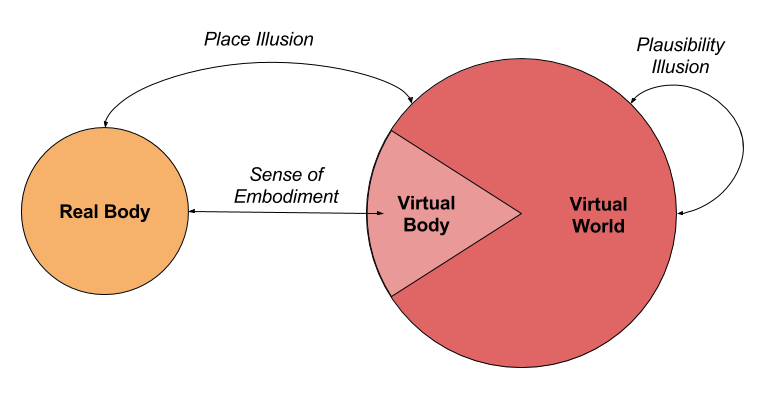
\includegraphics[width=\textwidth]{piPsiSoeDiagram.png}
\caption{Caption}
\label{fig:piPsiSoeDiagram}
\end{figure}

\todo[inline]{
Fill in caption.
Virtual body is just a particular case of the virtual world and in regards to PI, it is just a part that we ALWAYS perceive when we perform some sensorimotor actions.
Psi is VW on VW and VW on VB and VB on VB.
PI is RB on VW and RB on VB.
SoE is RB on VB.
}

\section{The Virtual Constraints Problem}
\label{sec:virtualContraintsProblem}

We now seek to describe the problem that we are addressing in this work, that is, the Virtual Constraints Problem, using the concepts that we have just defined. Furthermore, we shall use the theory to argue why the adjusted hand control model is an approach worth exploring.

The Virtual Constraints Problem has two conflicting goals:

\begin{enumerate}
\item Make the virtual body respect the virtual environment physics.
\item Preserve the connection between the user's real body and the virtual body.
\end{enumerate}

The first goal is mainly related to Psi. As previously discussed, the user knows how real bodies interact with the environment and if their virtual body does not interact with the environment like they know real bodies do, this dissonance will remind the user of the irreality of the virtual experience. If the world we are perceiving doesn't work like the real world, the world we are perceiving cannot be the real world, thus what is apparently happening is not really happening, which implies a break of Psi.

The second goal has to do with the PI, Sense of Self-Location and the Sense of Agency. If the virtual body separates from the real body, the user might stop perceiving themselves to be occupying the space where the virtual body is, which implies losses in PI and the Sense of Self-Location in the virtual body. In the case of Sense of Agency, the loss would happen if the separation of the virtual body from the real body happens in a way that makes the user stop feeling in control of the virtual body.

We can see that the conflicting goals of the Virtual Constraints Problem bring to light conflicting requirements between Psi and some of the components of SoE.

\todo[inline]{Connecting sentence? Something about the next section saying that there the theory suggests there is hope in the adjusted hand control model.}

\todo[inline]{In relation to PI: adjusted hand control models add SCs (but they don't necessarily remove SCs?)}

\subsection{The Rubber Hand Illusion}
\label{subsec:rubberHandIllusion}

Considering Kilteni et al.'s explanation of SoE, one would think that using adjusted hand control models would make SoE difficult. In terms of the aforementioned components of SoE, one might expect that separating the virtual hand from the real hand would have a direct negative impact on the Sense of Self-Location because the virtual hand is not where the user feels their own hand to be through proprioception. It would likely also affect the Sense of Agency, by making the virtual hand not follow the user's movements exactly, we are taking part of the control away from them in comparison with a 1 to 1 control method. Thirdly, in regards to the Sense of Ownership, it would be harder for the user to believe that the virtual hand is theirs if they don't see it where they feel their own hand to be.

The well-known Rubber Hand Illusion, originally reported in \parencite{Botvinick1998}, and other related experiments suggest that these issues might not be a problem after all. Experiments demonstrating this illusion typically have the following setup: the test subject places their right arm behind a panel that hides it from their view, a fake rubber arm is placed within their view, aligned with their real arm. The fake and real hands are synchronously stroked with paintbrushes in the same way for a period of time. When the subjects are asked to point towards their right arm with their eyes closed, typically they point toward the rubber arm, effect know as proprioceptive drift. In questionnaires after the experiment, subject reports showed a degree of attribution of the rubber hand \parencite{Botvinick1998} and when the rubber hand was injured subjects reacted as in anticipation of pain \parencite{Armel2003}. The reported attribution of the fake hand and the anticipation of pain signify a Sense of Ownership towards the fake hand.

\parencite{Sanchez-Vives2010} replicated the illusion with a virtual reality setup by making the virtual hand follow the movements of the subject's real hand, instead of using the sense of touch to induce the illusion, and found both proprioceptive drift and a degree of attribution of the virtual hand. These illusions map with the concepts of Sense of Place and Sense of Ownership that we pursue with our virtual hands.

\parencite{Kilteni2012}'s components of Sense of Embodiment seem to be found in the the Rubber Hand Illusion family of experiments and their similarity to the virtual hand - real hand separation produced by adjusted hand control models suggests that the results are transferable to our problem.

\subsection{From Where Should We Sense?}
\label{subsec:sensePerspective}

In real life, our body determines the "perspective" of our senses, we sense from our body: what we see is restricted by the position of our eyes, we can only feel an object with our touch if we can reach it with our hands. In Virtual Reality one has the option to restrict our senses either with the real body or with the virtual body. 

Imagine the case where a user moves their real head to a position that corresponds to somewhere inside a virtual object. If the virtual body is constrained by the virtual environment, it will separate from the real body at the surface of the virtual object. At this point, if the sense perspective is restricted to the virtual body, the user will see from the perspective of the virtual body, but if the sense perspective is restricted by the real body, the user will see from inside of the virtual object. 

The first behavior is the most coherent one and should benefit the Sense of Ownership of the virtual body because it connects the virtual senses of the user to it instead of to their real body. At the same time, the Sense of Self-Location would be challenged by the conflicting signals between our proprioception and our sight.

The second behavior would produce a break in Psi because seeing from inside of a solid should not match anyone's expectations about the worlds possibilities. It could also be argued that it would impact PI negatively, since from that situation we might be able to see our body from outside of it, which is not something our normal SCs would allow.

We would remiss if we didn't mention that at least in regards to the sense of sight, the first behavior might fall under what is generally considered a bad practice by the VR software development community. Specifically, it is discouraged to move the camera in any way that doesn't match the user's head movements because it is thought to produce discomfort in the user \parencite{UnityCamera, OculusCamera}. This would be an issue that would have to be considered in much greater detail if the focus of this work wasn't on the control of the hands.

\todo[inline]{Relationship between SoE and PI. Disembodying user. Rewrite.}

\section{Critiques of Movement Interaction}
\label{sec:critiquesMovementInteraction}

\parencite{Norman2010} rejects the claim that current gestural interfaces are Natural User Interfaces: "user interfaces where the interaction is direct and consistent with our ‘natural’ behaviour" \parencite{HvasMortensen2017}. Norman reminds us that the strength of a user interface is determined by how easy it is to remember the actions that are possible and how to invoke them. He points out that due to the ephemeral nature of gestures, when a gesture does not produce any response or produces an undesired one, the user lacks feedback that that they can use to learn to perform the gesture ‘correctly’.

Gilles argued in \parencite{Gillies2014} that if movement interfaces are non-representational, that is, if they implement the Sensorimotor Contingencies that we know from the real world, Norman's arguments might not apply. In \parencite{Gillies2016} however, he acknowledges that when the SCs implemented in the interfaces are only similar to the real-world SCs, they start to become representational and Norman's arguments regain their weight. An example of this provided by Gilles in the context of VR is "walking in place" as a locomotion control method.

In regards to unadjusted hand control models, since the mapping between the real movements of the user and the virtual movements is 1 to 1, these arguments need not be a concern, but this is less clear when it comes to adjusted hand control models because the virtual hands can separate from the user's real hands, which could be thought to make the control less intuitive. However, we would argue that because adjusted hand control models can still provide a sensorimotor feedback loop \parencite{Gillies2014} that matches our knowledge about how real bodies are restricted in their movement by physical objects around them, the issues that have been pointed out should not be a problem.

In a broad sense, the tracked controllers that the users hold in their real hands and use to control the virtual hands are part of the interface. In Chapter \ref{chap:introduction} we covered the differences between the controllers of the HTC Vive, the Oculus and the PS VR and we noted that the Oculus Touch controllers were the ones that had the most input mechanisms that could be used to control virtual fingers with movements of the real fingers. However, the user has to perform reduced movements with their real fingers that correspond to full movements with the virtual fingers, in the case of the triggers, which have analogue input, a continuous mapping between the movement of the real fingers and the virtual fingers is possible, which allows the sensorimotor feedback loop mentioned by Gilles, but in the case of the capacitive sensors, the user doesn't have a way of feeling that their fingers are about the trigger a state change until the state has triggered. These problems would of course not exist with the use of data gloves like the Manus VR Gloves since the gloves can track the movement of the fingers completely.

On the software side, both Facebook Spaces \parencite{facebookSpaces} and Oculus First Contact \parencite{firstContact}, which use and showcase the possibilities of Oculus Touch controllers, use representational movement interaction. Buttons, both when they are diegetic and when they are part of a GUI, can only be pressed with the the index finger, and only when it is extended. The virtual hands only collide with virtual physical objects in certain poses, like with a closed fist. Because the movement control these games is more representational, it requires more attention from the user and it simple hand gestures can become rather complicated when thought of in terms of combinations of input. The problem is that we want to minimize the amount of attentional resources that the user needs to focus on the controllers because they are part of the real world and not of the virtual reality, which is where we want the users to have their attention (Witmer and Singer relate presence to attention allocation and defined presence as partly determined by involvement \parencite{Schuemie2001}).

\section{\textit{Encore}: Current VR Games}
\label{sec:soaRevisited}

Armed with a theoretical framework, we can revisit the games discussed in Chapter \ref{chap:introduction} and evaluate them in terms of PI, Psi and SoE, mostly focusing on the hands. The reader should bear in mind that these are subjective experiences and that what we present here are evaluations based on our own individual impressions. In order to obtain more reliable assessments, one should conduct tests with larger groups of subjects and use perhaps some of the existing questionnaires and tests that measure physiological and behavioral responses.

Job Simulator is our example of an unadjusted hand control model. It produces high PI and SoE because its 1 to 1 mapping of the hands to the controllers means that the movements that the user wants to do with their virtual hands are exactly the same as the ones that they have to do with their real hands (within the limits of the hardware system). Where one might take issue with Job Simulator's hands is in regards to Psi. The hands can penetrate immovable virtual objects that the user will easily recognize from real life and expect to not allow their hands to go through (recall Figure \ref{fig:jobSimStaticProblem} in Chapter \ref{chap:introduction}). For analogous reasons, the fact that the hands disappear when holding objects in Job Simulator can also produce breaks in Psi.

\todo[inline]{Relate PI only to SCs! In both cases when it comes to the hands, we don have sensory input, so there is no PI? When it comes to spatial presence, refer to Sense of Self-Location.}

It should be noted however, that the experience of playing Job Simulator is hardly objectionable even though from a rational perspective the world doesn't work like the real world. Its cartoonish, low fidelity visual aesthetics and humor elicit the required level of suspension of disbelief and set the right expectations in the user (see \parencite{Nowak2003, Argelaguet2016} on how the visual fidelity level can influence user's expectations and affect their experience in VR). In fact, the game frequently surprises players with the level of detail in the environment in terms of interactibility \parencite{Schwartz2017}.

\todo[inline]{Mention \parencite{Schubert1999}'s presence correlated with predictibility and explorability?}

Wilson's Heart's hands don't quite fit in the adjusted hand control model, but the way they work provides useful information that is relevant for the Virtual Constraints Problem. As discussed in Chapter \ref{chap:introduction}, in this case the virtual hands follow the real user's hands without separating from them until an interaction with a virtual object is triggered, generally by input produced by the user's real fingers using the analogue triggers or the capacitive sensors in the Oculus Touch. When said interactions happen, the hands snap to a pose that is predefined for each object. In most cases, these transitions from following the tracking devices exactly to largely ignoring the tracking data are quite natural and the separation wasn't noticeable, so in terms of Sense of Self-Location this works well. In terms of Sense of Agency, however, the fact that the interactions with virtual objects were mostly limited to the predefined poses for each object did have a negative effect. While there are no interactions that override the user input, the Sense of Self-Location, but specially the Sense of Agency are enhanced by the amount of control over the fingers that the Oculus Touch controllers allow.

The physical interaction between the virtual hands and the environment is - aside from the predefined interactions - far more limited than in Job Simulator: the hands go through many objects or have to be in specific finger poses to be able to physically impact the objects, which works against producing Psi because the user is constantly reminded these differences with the real world. This is aggravated by the fact that Wilson's Heart, although restricted in colors to greyscale, has a much more realistic aesthetic. In the same way that having a low fidelity style worked in favor of Job Simulator, this can work against Wilson's Heart.

\begin{figure}[h]
\centering
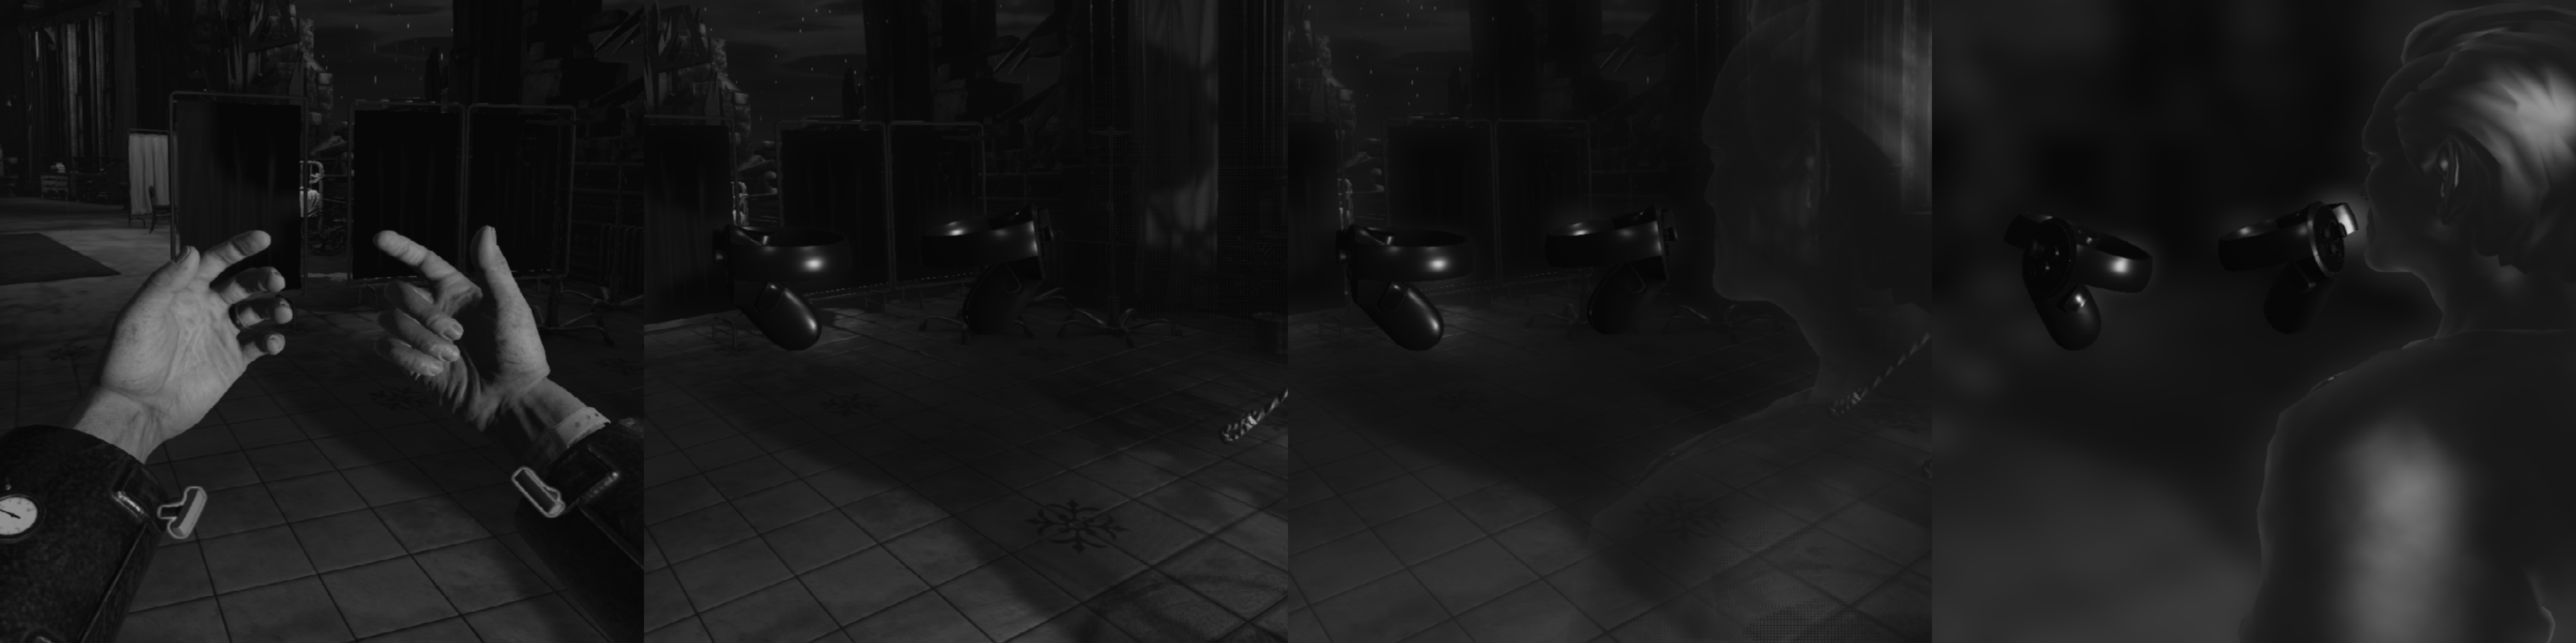
\includegraphics[width=\textwidth]{Sequences/WilsonsHeart/wilsonOutOfBodyExperience.png}
\caption{Sequence showing an "out of body experience" in Wilson's Heart: the sense perspective is not restricted by the virtual body.}
\label{fig:wilsonOutOfBody}
\end{figure}
\todo{Add link to gif}

Wilson's Heart provides a great example of sense perspective restricted to the real body instead of the virtual body. If the player moves too far from the virtual body, they will be disembodied, the world becomes blurry, the virtual body turns transparent and the Oculus Touch controllers become visible. This approach opts to break the SoE more abruptly in order to clearly establish the limits of what the player is allowed to do.